\documentclass{standalone}
\usepackage{tikz}
\tikzset{block/.style = {draw, fill=white, very thick, rectangle, minimum height=1cm, minimum width=2cm}}
\begin{document}
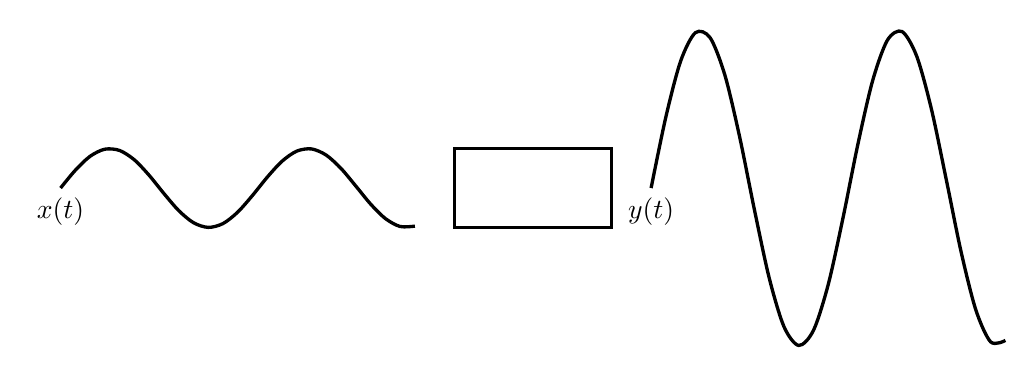
\begin{tikzpicture}[scale=2]
    \draw[-,very thick]plot[smooth, domain=-3:-0.75](\x,{0.25*sin(5*(\x+3) r)});
        \draw[-,very thick]plot[smooth, domain=0.75:3](\x,{1*sin(5*(\x-0.75) r)});
        \node[block](s)at(0,0){};
        \node[below]at(-3,0){$x(t)$};
        \node[below]at(0.75,0){$y(t)$};
\end{tikzpicture}
\end{document}